\chapter{Utiliser le code de contrôle}
\label{codeValidation}
%\minitoc

Epi Info 7 dispose d'un mécanisme de validation des données appelé \emph{Check Code}, ou code de contrôle. Le code de contrôle rend le formulaire plus intelligent : son comportement peut changer au cours de la saisie. Il permet notamment de calculer automatiquement des valeurs comme l'âge ou l'IMC, d'appliquer des sauts de questions, d'afficher des messages ou des questions à l'utilisateur pendant la saisie, de remplir des champs et de masquer des champs.
Le code de contrôle se construit à l'aide de boîtes de dialogue disponibles dans le module \module{créer questionnaires}. C'est à nous de programmer le comportement que nous voulons donner à notre questionnaire.

\section{Ouvrir l'éditeur de code de contrôle}

Pour accéder au code de contrôle, il faut d'abord ouvrir un formulaire :

\begin{enumerate}
\item Ouvrir Epi Info 7 et aller dans le module \module{créer questionnaires} ;
\item Dans la barre d'outils, cliquer sur \kw{Fichier} puis sur \kw{Ouvrir le projet}. Vous pouvez aussi utiliser le raccourci clavier \kw{Ctrl + O} ;
\item Aller dans le répertoire des projets d'Epi Info 7 et ouvrir le dossier de notre projet \var{COVID19}, créé au chapitre~\ref{creerQuestionnaire} (il faudra peut-être faire défiler la liste pour l'apercevoir) ;
\item Ouvrir le fichier \var{COVID19.prj}, par un double-clic ou en le sélectionnant puis en cliquant sur \kw{Ouvrir} ;
\item Une fois le formulaire ouvert, cliquer sur le bouton \kw{Code de contrôle}, qui ouvre l'éditeur de code de contrôle (\autoref{fig:editeurcodevalidation}).
\end{enumerate}

\begin{figure}[H]
	\centering
	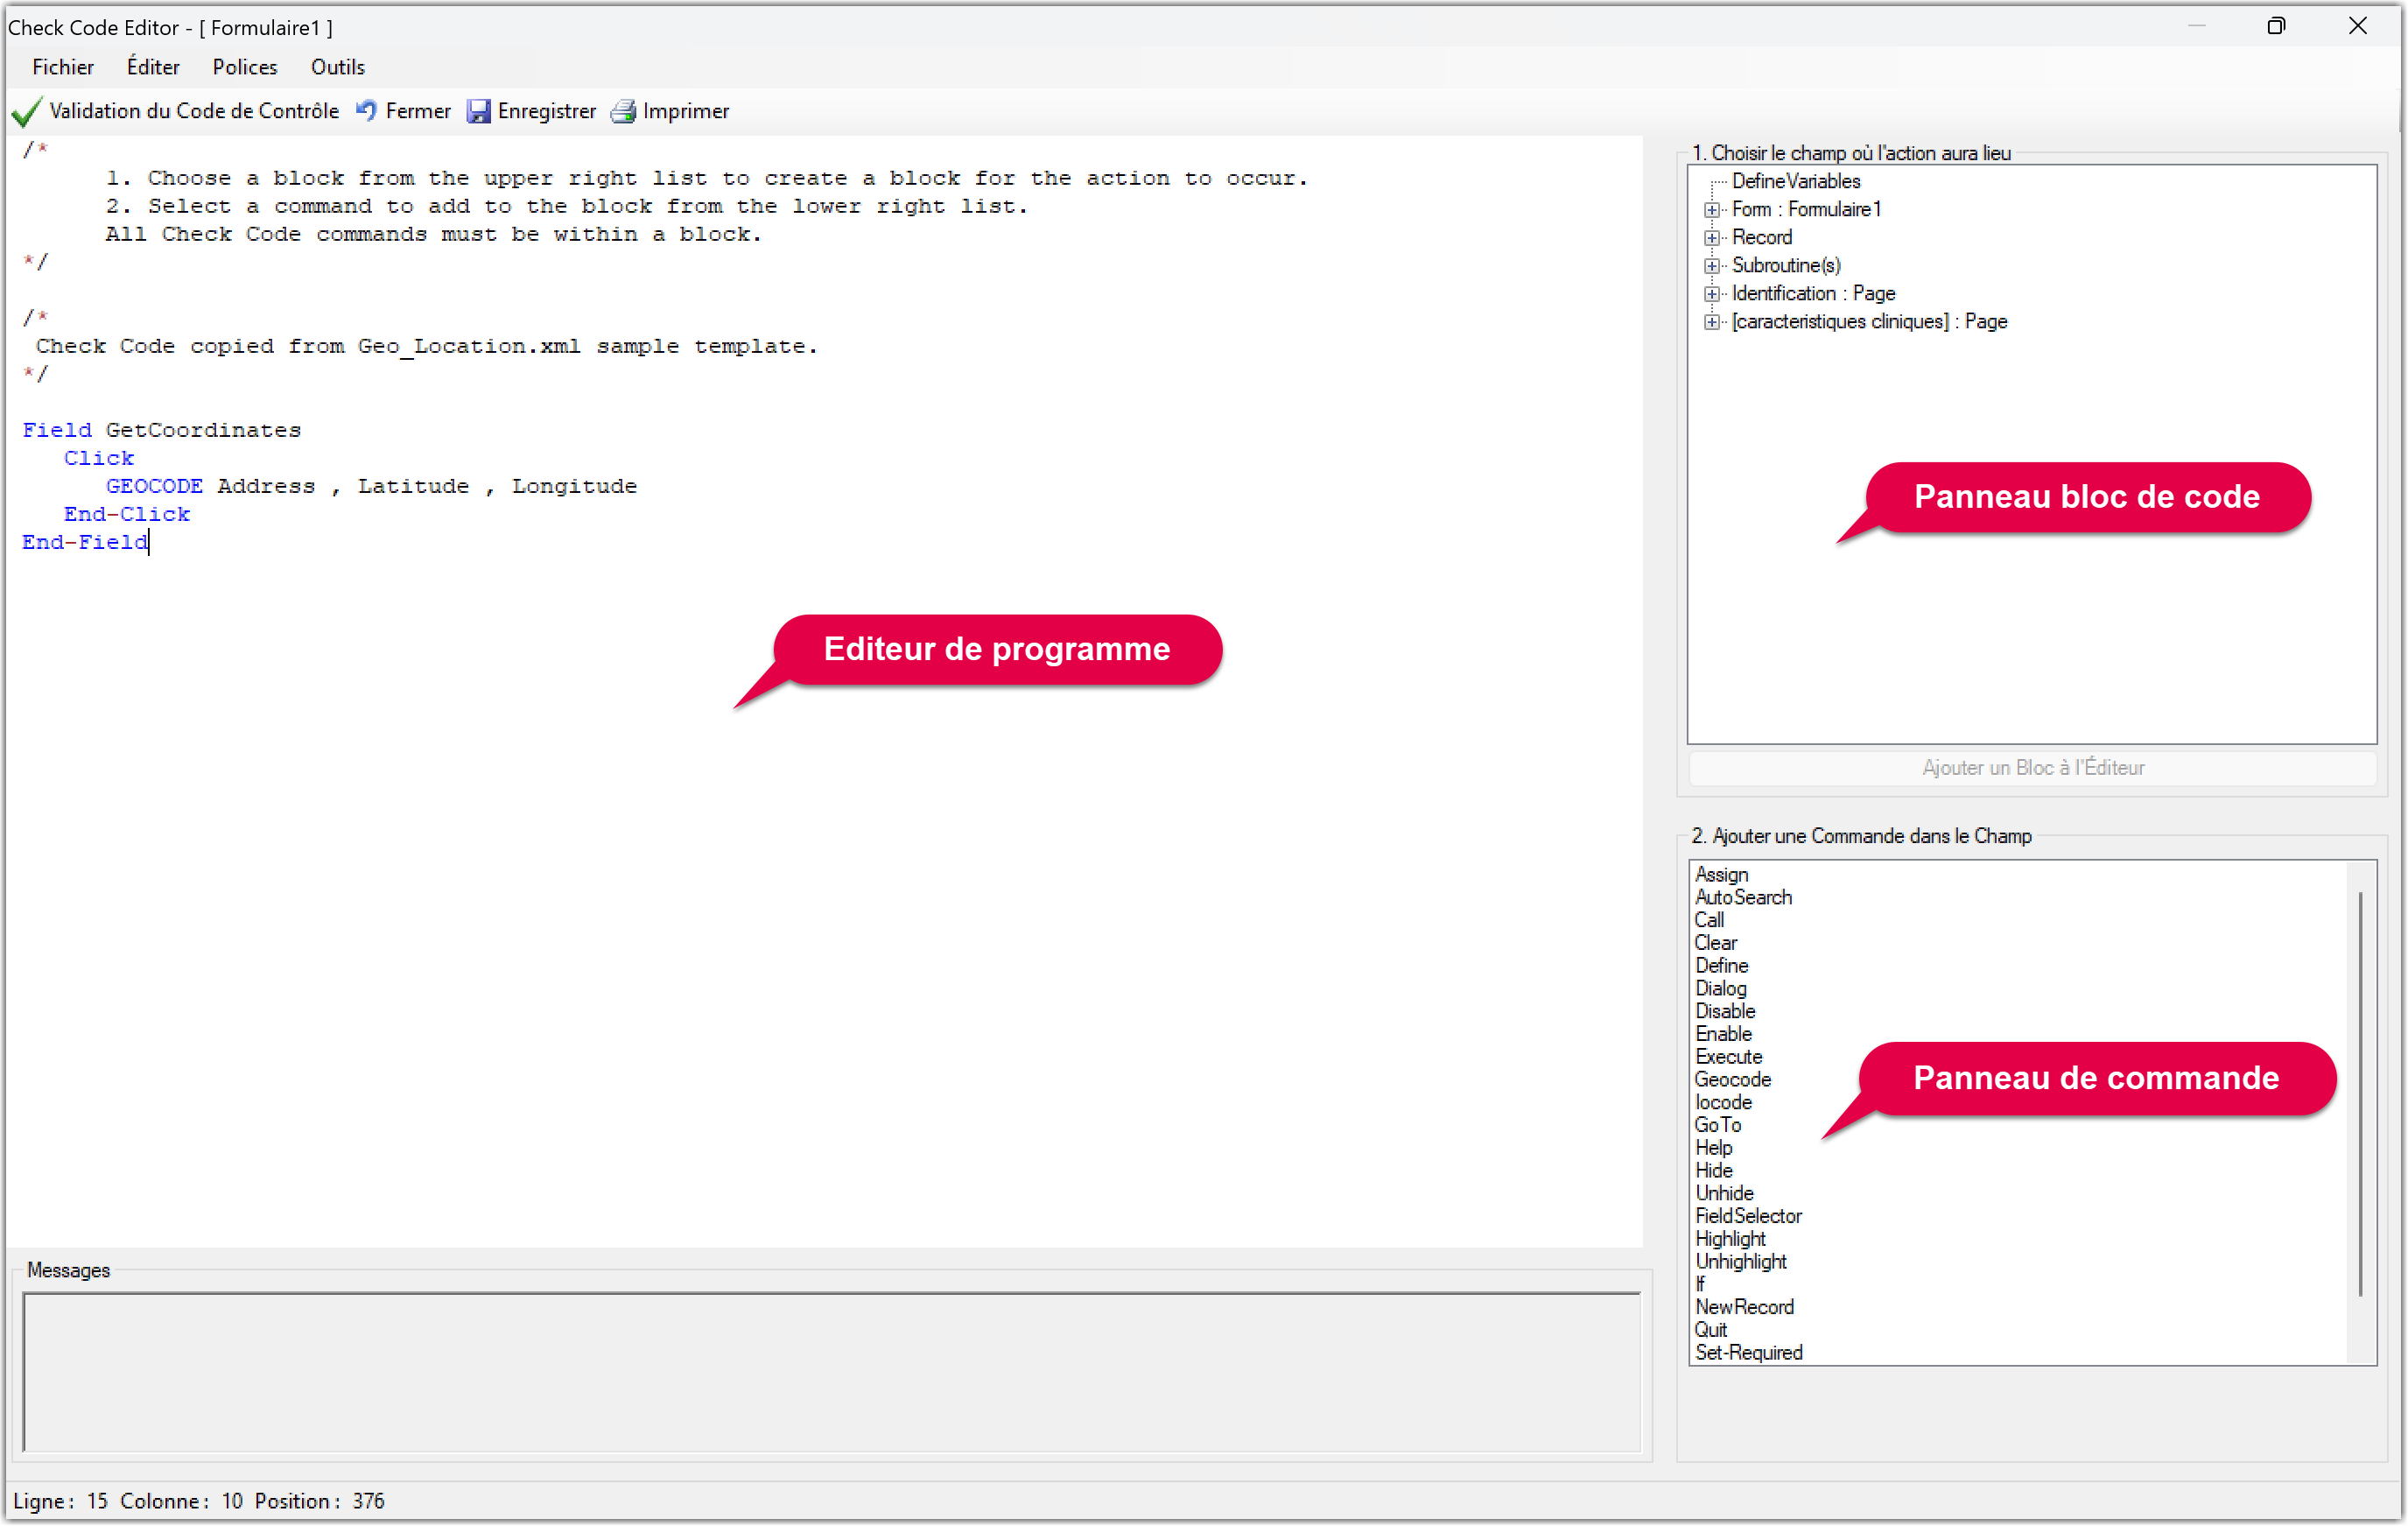
\includegraphics[width=\linewidth,height=0.4\textheight,keepaspectratio]{img/CodeValidation/editeurCodeValidation}
	\caption{Éditeur du code de contrôle}
	\label{fig:editeurcodevalidation}
\end{figure}

Tout code de contrôle doit être associé à un champ existant du formulaire. Les champs disponibles sont listés, page par page, dans le panneau \kw{Choisir le champ où l'action aura lieu}.

Le code de contrôle repose sur des événements : nous définissons le comportement des champs en fonction d'actions comme l'ouverture ou la fermeture du formulaire, l'ouverture ou la fermeture d'une page, l'entrée du curseur dans un champ (\commande{Before}) ou sa sortie (\commande{After}).

\begin{mybox}[colbacktitle=NOTE]{\faInfoCircle{} À RETENIR}
Dans l'éditeur, vous ne verrez pas l'intitulé de vos questions mais le nom des variables, c'est-à-dire ce que vous avez saisi dans \kw{Nom du champ}. D'où l'importance, une fois de plus, de bien nommer ses variables.
\end{mybox}

\section{Les principales commandes}

Dans ce chapitre, nous voulons calculer automatiquement l'âge de la personne enquêtée à partir de sa date de naissance et de la date de l'enquête. Epi Info 7 calcule la différence entre deux dates en années, en mois ou en jours, avec respectivement les fonctions \commande{YEARS()}, \commande{MONTHS()} et \commande{DAYS()}. De même, au lieu de calculer l'indice de masse corporelle (IMC) à la main, nous voulons le déduire du poids et de la taille. Rappelons que l'IMC est égal au poids en kilogrammes divisé par le carré de la taille en mètres. La taille étant saisie en centimètres, nous la divisons par 100 :
\[
\text{IMC} = \frac{\text{poids\_kg}}{\left(\text{taille\_cm}/100\right)^2}
\]

Voici les commandes du code de contrôle que nous utiliserons le plus :

\begin{itemize}[label=\ding{45}]
	\item \commande{DEFINE} (Définir) : crée une nouvelle variable ;
	\item \commande{ASSIGN} (Attribuer) : affecte à une variable le résultat d'une opération arithmétique ou d'une expression de texte ;
	\item \commande{HIDE} (Masquer) : masque un champ pour le rendre invisible ;
	\item \commande{UNHIDE} (Afficher) : rend visible un champ masqué auparavant ;
	\item \commande{DISABLE} (Désactiver) : désactive un champ. Un champ désactivé n'accepte aucune saisie et sort de l'ordre de tabulation ;
	\item \commande{ENABLE} (Activer) : réactive un champ désactivé auparavant ;
	\item \commande{IF} (Si) : définit une condition et ce qui doit se passer si elle est remplie. Une autre action peut être prévue après l'instruction \commande{ELSE} (Sinon) ;
	\item \commande{GOTO} (Aller à) : seul ou dans une instruction If, envoie le curseur vers un champ ou une page ;
	\item \commande{CLEAR} (Effacer) : vide le champ indiqué, comme s'il n'avait jamais été rempli ;
	\item \commande{DIALOG} (Boîte de dialogue) : affiche un message à l'utilisateur.
\end{itemize}

\section{La commande Assign}

Dans notre questionnaire, l'âge doit être déduit de la date de naissance et de la date de l'enquête, et l'IMC du poids et de la taille. Nous voulons donc affecter aux variables \var{age} et \var{imc} une formule de calcul : c'est le rôle de la commande \commande{ASSIGN}.

Une fois dans l'éditeur de code de contrôle, procéder comme suit pour remplir automatiquement le champ \var{age} (\autoref{fig:creercodevalidationage}) :

\begin{enumerate}
	\item Dans le panneau des blocs de code, cliquer sur le $+$ à côté de \kw{Identification : Page} pour déplier les champs de la page Identification (étape 1) ;
	\item Cliquer sur le $+$ à gauche de la variable \var{age} (étape 2) ;
	\item Cliquer sur \commande{After} (étape 3) : l'action aura lieu à la sortie du champ ;
	\item Cliquer sur \kw{Ajouter un bloc} pour ajouter le bloc de code dans l'éditeur de programme (étape 4) ;
	\item Dans le panneau des commandes, cliquer sur la commande \commande{ASSIGN}. Une fenêtre apparaît (étape 5) ;
	\item Cliquer sur la flèche déroulante \kw{Assigner variable} et choisir la variable \var{age} (étape 6) ;
	\item Dans la partie \kw{Expression}, cliquer sur le petit rectangle $f(x)$ (étape 7) ;
	\item Dans le menu qui s'ouvre, aller à \kw{Fonctions Date} (étape 8) ;
	\item Dans le dernier sous-menu, choisir la fonction \commande{YEARS()} (étape 9).
\end{enumerate}

\begin{figure}[H]
	\centering
	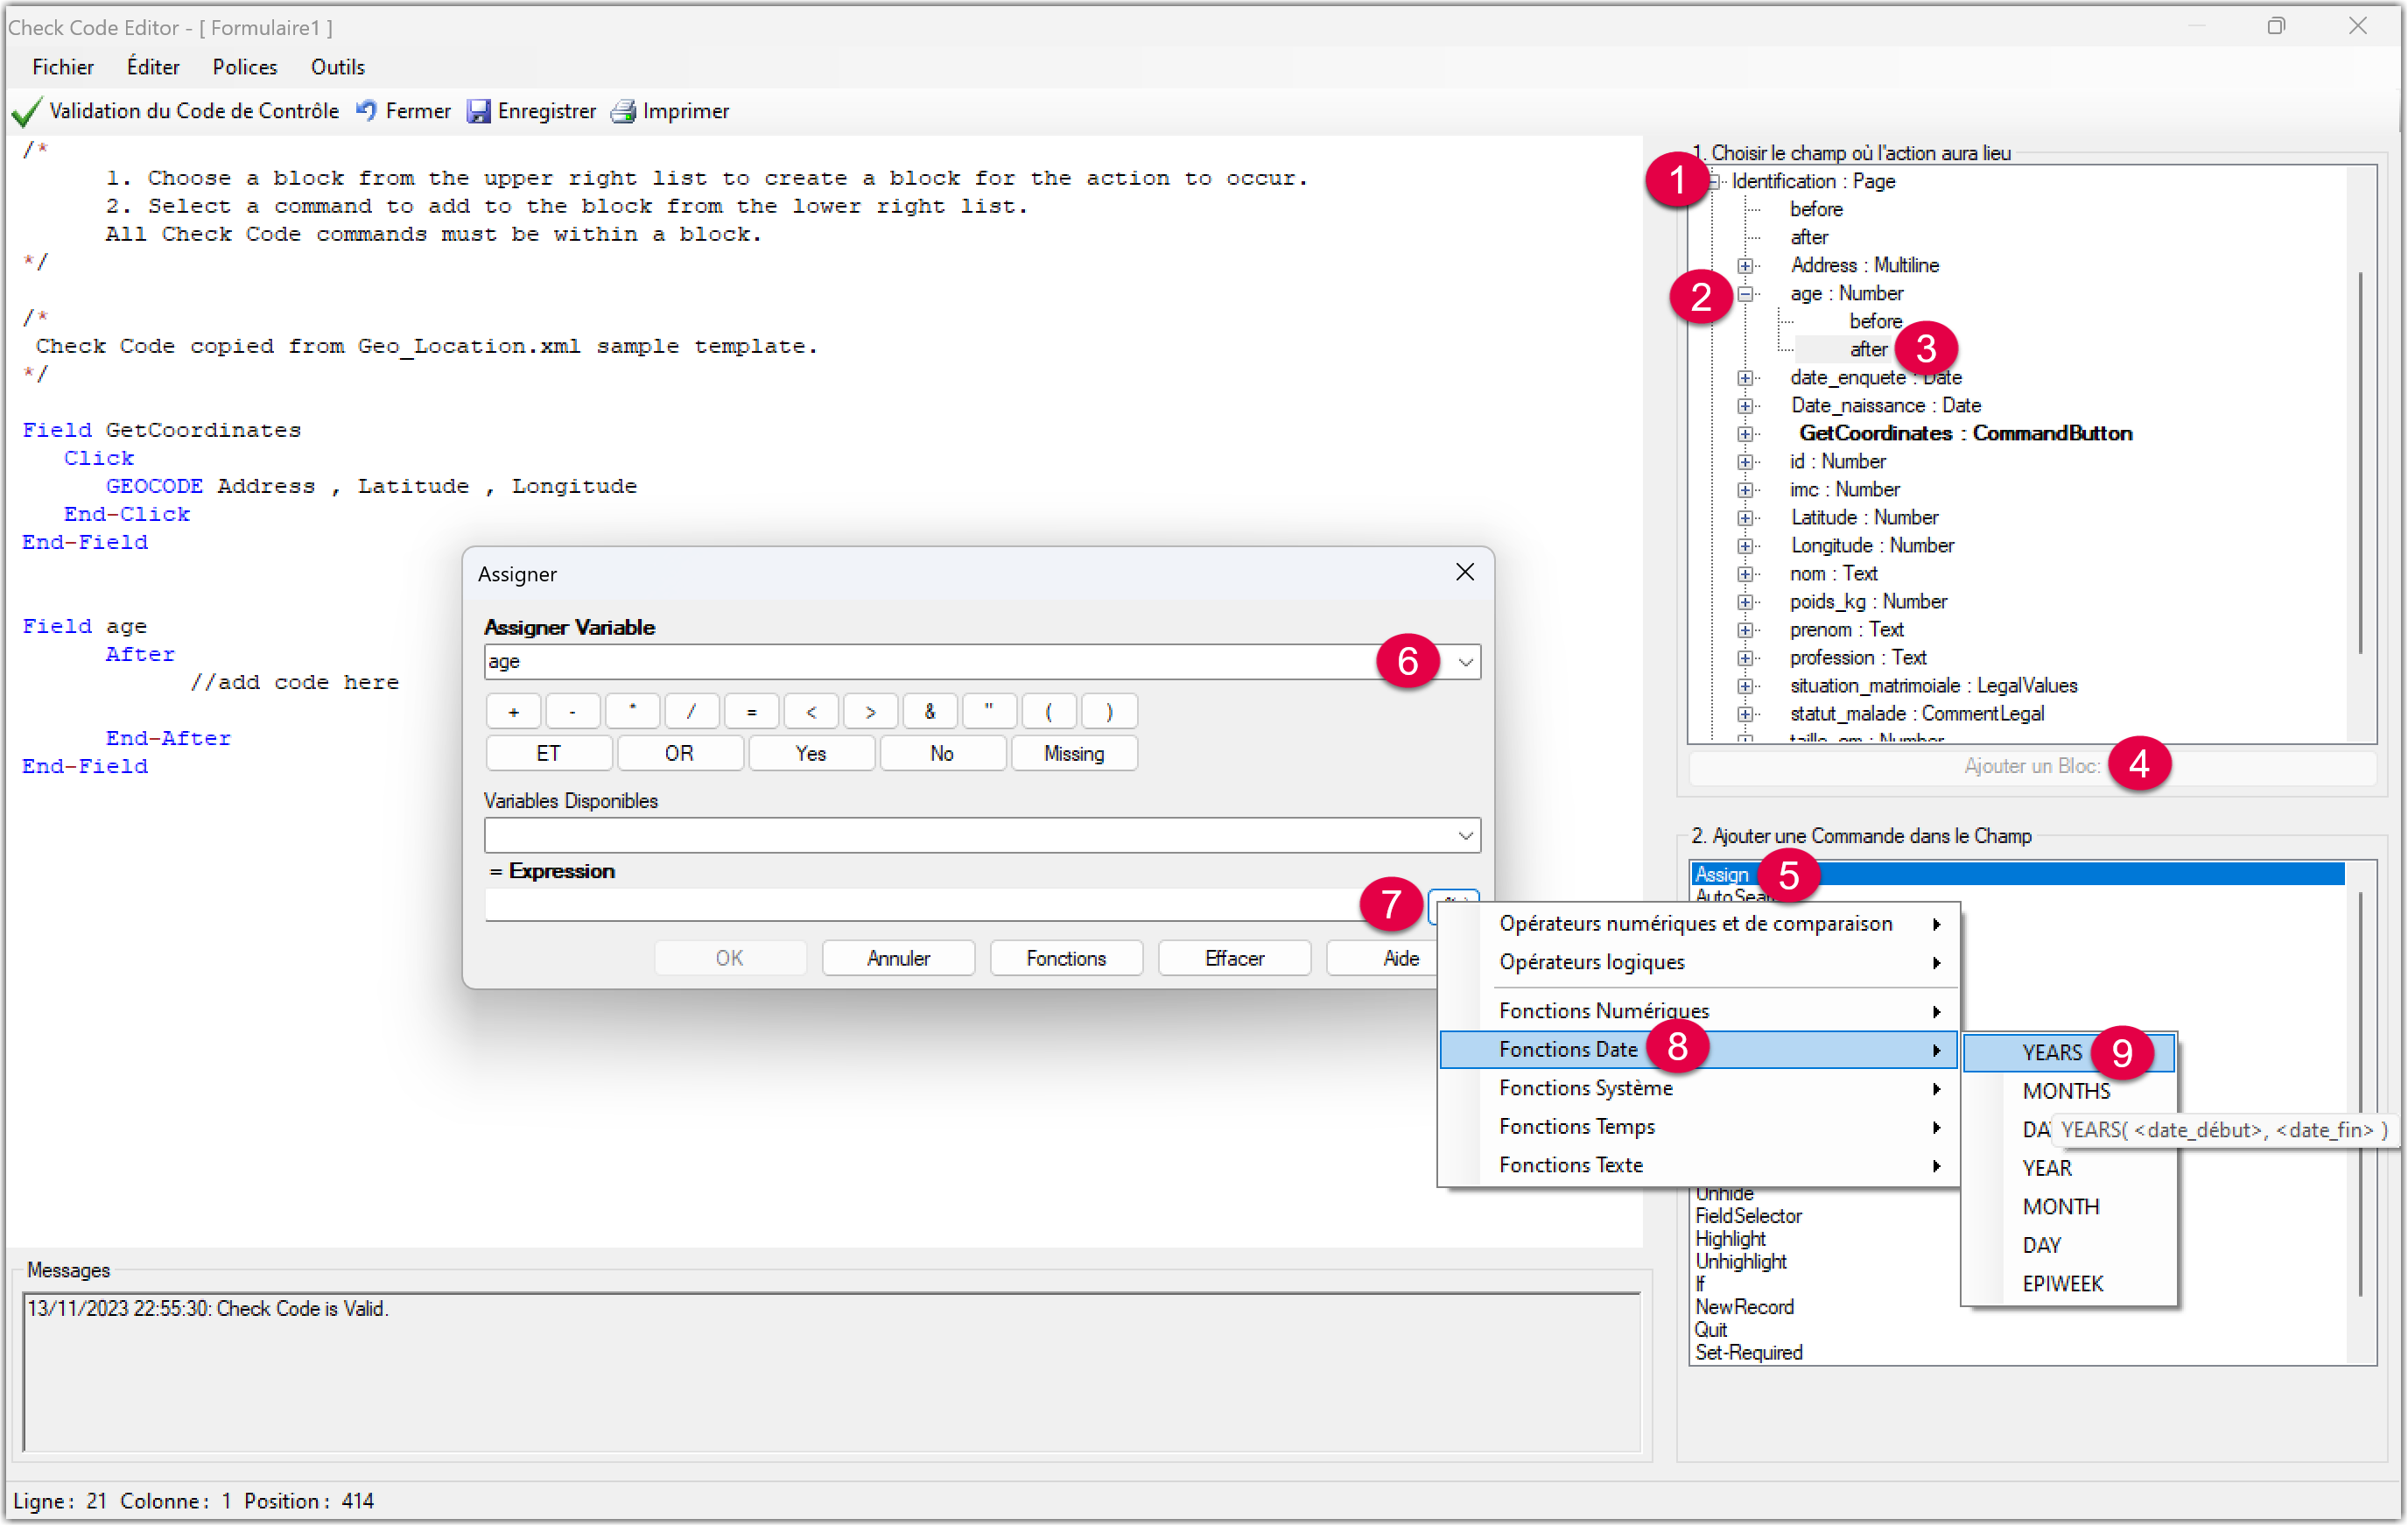
\includegraphics[width=\linewidth,height=0.4\textheight,keepaspectratio]{img/CodeValidation/creerCodeValidationAge}
	\caption{Création d'un code de contrôle pour le champ âge}
	\label{fig:creercodevalidationage}
\end{figure}

L'expression générique de la fonction s'affiche alors : \commande{YEARS(date\_debut, date\_fin)}. Nous la complétons avec nos variables (\autoref{fig:ecrituredelalogiqueage}) :
\begin{enumerate}
	\item Double-cliquer sur \var{date\_debut} pour le sélectionner ;
	\item À l'aide de la flèche déroulante \kw{Variables disponibles}, choisir la variable \var{date\_naissance} ;
	\item Double-cliquer sur \var{date\_fin} ;
	\item Dans la liste \kw{Variables disponibles}, choisir la variable \var{date\_enquete} ;
	\item Valider le tout par \kw{OK} (\autoref{fig:codeassign}).
\end{enumerate}

\begin{figure}[H]
	\centering
	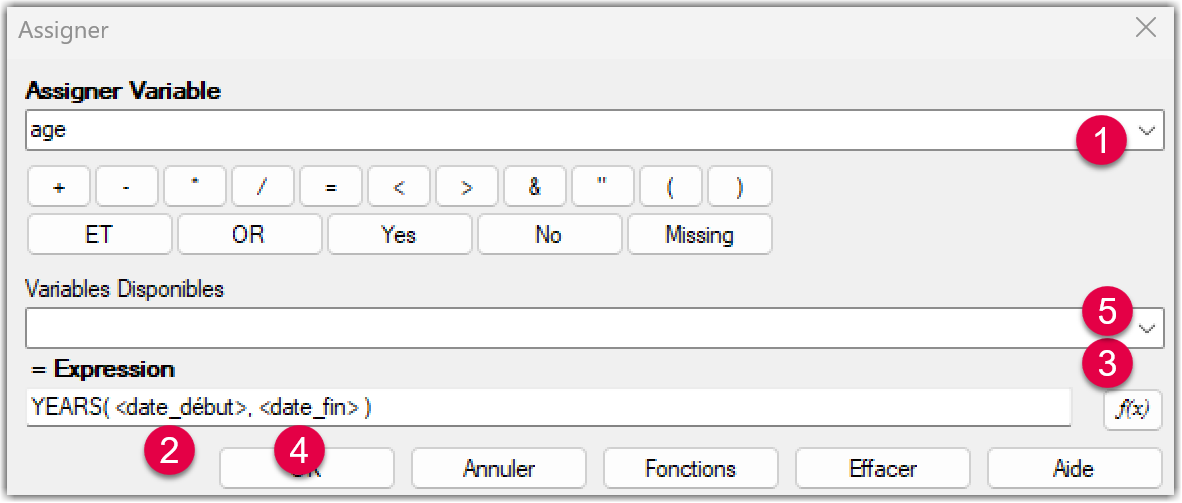
\includegraphics[width=\linewidth,height=0.4\textheight,keepaspectratio]{img/CodeValidation/ecritureDeLaLogiqueAge}
	\caption{Écriture de l'expression de la fonction YEARS()}
	\label{fig:ecrituredelalogiqueage}
\end{figure}

\begin{figure}[H]
	\centering
	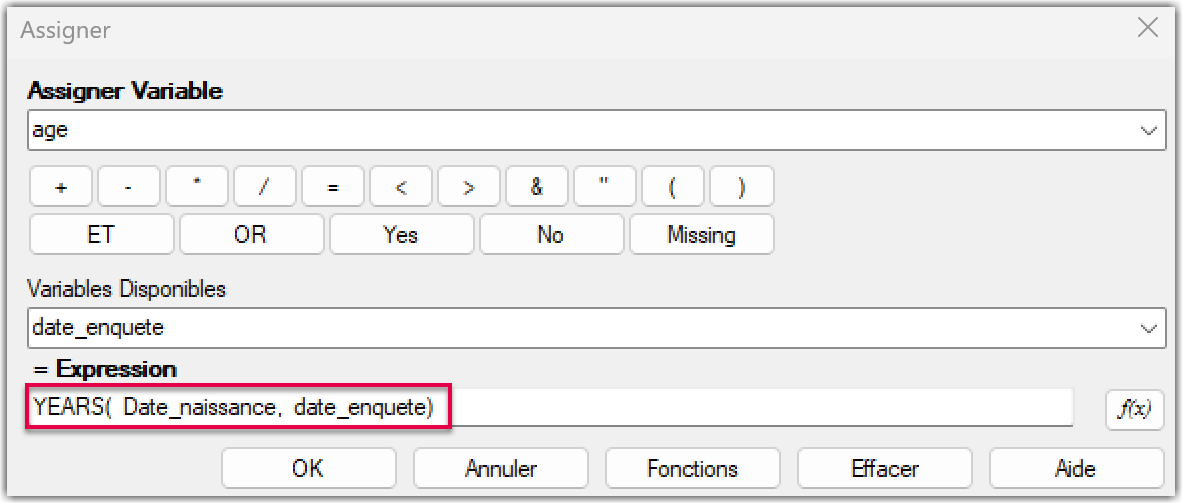
\includegraphics[width=\linewidth,height=0.4\textheight,keepaspectratio]{img/CodeValidation/codeAssign}
	\caption{Fonction YEARS()}
	\label{fig:codeassign}
\end{figure}

Après validation, le code apparaît dans l'éditeur de programme (\autoref{lst:assign}, page~\pageref{lst:assign}). Il reste à vérifier que le code est valide en cliquant, en haut à gauche, sur \kw{Valider le code de contrôle}\footnote{Un message s'affiche en bas, dans la zone \kw{Messages}, avec la date, l'heure et la mention \commande{Check Code is Valid} si le code est valide. Sinon, une erreur est signalée.}, puis à l'enregistrer en cliquant sur \kw{Enregistrer}.

\begin{tcolorbox}[drop lifted shadow]
	\begin{lstlisting}[language=EPIscript, style=mystyle, caption={Utilisation de la fonction YEARS() avec la commande ASSIGN}, label=lst:assign]
Field age
	After
		//add code here
		ASSIGN age = YEARS(date_naissance, date_enquete)
	End-After
End-Field
	\end{lstlisting}
\end{tcolorbox}

Nous créons de la même manière le code de contrôle de la variable \var{imc} (\autoref{fig:assignationimc}) :

\begin{enumerate}
	\item Dans le panneau des blocs de code, chercher la variable \var{imc}, qui se trouve sur la page Identification du formulaire ;
	\item Cliquer sur le $+$ à gauche de la variable \var{imc}, puis sur \commande{After} ;
	\item Cliquer sur \kw{Ajouter un bloc} ;
	\item Cliquer sur la commande \commande{ASSIGN} dans le panneau des commandes et choisir la variable \var{imc} ;
	\item Dans la partie \kw{Expression}, écrire la formule de l'IMC en vous aidant de la liste \kw{Variables disponibles}. N'oubliez pas de diviser la taille par 100 pour la convertir en mètres, puisque nous avons choisi de recueillir les tailles en centimètres ;
	\item Valider par \kw{OK} : le code apparaît dans l'éditeur de programme (\autoref{lst:imc}, page~\pageref{lst:imc}) ;
	\item Vérifier la validité du code en cliquant sur \kw{Valider le code de contrôle} ;
	\item Enregistrer le code en cliquant sur \kw{Enregistrer}.
\end{enumerate}

\begin{figure}[H]
	\centering
	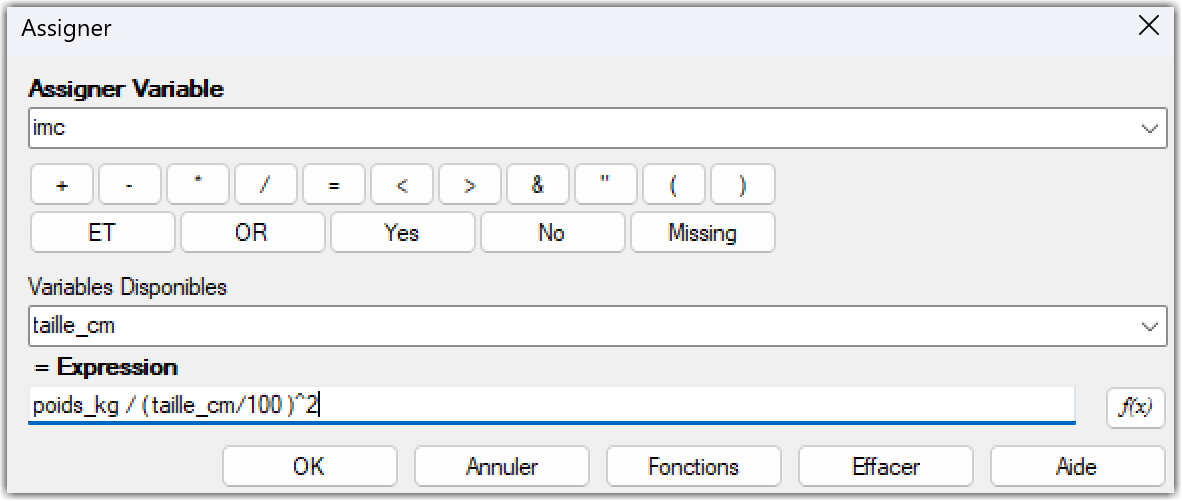
\includegraphics[width=\linewidth,height=0.4\textheight,keepaspectratio]{img/CodeValidation/assignationIMC}
	\caption{Création du code de contrôle de la variable imc}
	\label{fig:assignationimc}
\end{figure}

\begin{tcolorbox}[drop lifted shadow]
	\begin{lstlisting}[language=EPIscript, style=mystyle, caption={Code d'assignation de la variable imc}, label=lst:imc]
Field imc
	After
		//add code here
		ASSIGN imc = poids_kg/(taille_cm/100)^2
	End-After
End-Field
	\end{lstlisting}
\end{tcolorbox}

\begin{mybox}[colbacktitle=IMPORTANT]{\faExclamationCircle{} IMPORTANT}
	\begin{itemize}[label=\ding{97}, font=\color{IMPORTANT}]
	\item En informatique en général, et dans Epi Info en particulier, les opérations arithmétiques s'écrivent $+$, $-$, $*$ et $/$ pour l'addition, la soustraction, la multiplication et la division. Le symbole \textcolor{IMPORTANT}{\texttt{\^{}}} représente la puissance ;
	\item Vérifiez toujours la validité du code ;
	\item Enregistrez toujours le code avant de quitter l'éditeur de code de contrôle.
\end{itemize}
\end{mybox}

\section{Les commandes If, Dialog, Clear et GoTo}

La commande \commande{IF} est utilisée en algorithmique et dans de nombreux langages de programmation pour exécuter une action sous condition. Elle s'emploie le plus souvent sous la forme \commande{IF} (condition) \commande{THEN} (action) \commande{ELSE} (autre action), soit : \og si la condition est vérifiée, exécuter ce bloc de code ; sinon, exécuter cet autre bloc \fg{}. Passons sans plus tarder à la démonstration.

Nous allons écrire un code simple qui nous alerte si nous saisissons par erreur une taille inférieure ou égale à 0~cm ou supérieure ou égale à 300~cm. Le code affiche alors une fenêtre intitulée \og Attention ! \fg{} avec le message \question{La taille saisie est incorrecte}, efface la valeur saisie et replace le curseur dans le champ pour une nouvelle saisie. Procédons comme suit (\autoref{fig:codeconditionsi}, page~\pageref{fig:codeconditionsi}) :

\begin{enumerate}
	\item Ouvrir l'éditeur de code de contrôle ;
	\item Dans le panneau des blocs de code, chercher la variable \var{taille\_cm}, située sur la page \kw{Identification} du formulaire ;
	\item Cliquer sur le $+$ pour déplier les événements de cette variable ;
	\item Cliquer sur \commande{After} puis sur \kw{Ajouter un bloc} ;
	\item Dans le panneau des commandes, cliquer sur la commande \commande{IF}. Une fenêtre s'ouvre ;
	\item Écrire la condition dans la case \kw{Condition Si}. On peut s'aider de la liste \kw{Variables disponibles} et du bouton de fonctions $f(x)$ ;
	\item Dans la partie \kw{Alors}, indiquer le code à exécuter lorsque la condition est vérifiée. Ici, nous ajoutons les commandes \commande{DIALOG}, \commande{CLEAR} et \commande{GOTO} en cliquant à chaque fois sur le petit symbole de document, dans le coin droit de la partie \kw{Alors} (étape \textcolor{IMPORTANT}{\Large \ding{204}} de la \autoref{fig:codeconditionsi}) ;
	\item On peut aussi utiliser la partie \kw{Sinon} (\commande{ELSE}) pour indiquer le code à exécuter lorsque la condition n'est pas vérifiée ;
	\item Cliquer sur \kw{OK} pour afficher le code créé dans l'éditeur de programme, puis le valider et l'enregistrer.
\end{enumerate}

\begin{figure}[H]
	\centering
	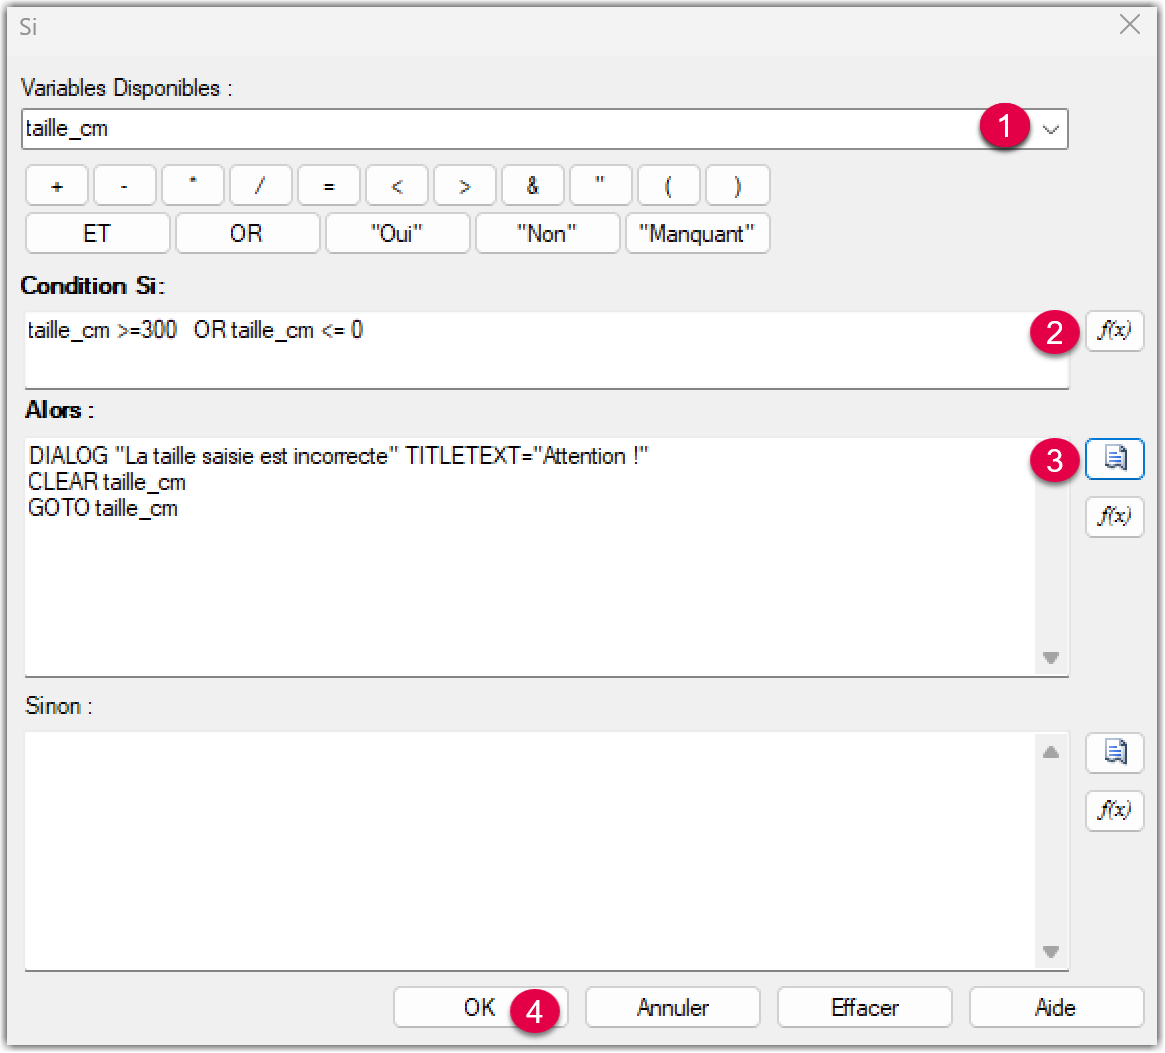
\includegraphics[width=\linewidth,height=0.4\textheight,keepaspectratio]{img/CodeValidation/codeConditionSi}
	\caption{Utilisation de la commande IF}
	\label{fig:codeconditionsi}
\end{figure}

Le code obtenu est présenté dans le \autoref{lst:dialog}, page~\pageref{lst:dialog}.

\begin{tcolorbox}[drop lifted shadow]
	\begin{lstlisting}[language=EPIscript, style=mystyle, caption={Code de contrôle de la variable taille\_cm}, label=lst:dialog]
Field taille_cm
	After
		//add code here
		IF taille_cm >= 300 OR taille_cm <= 0 THEN
			DIALOG "La taille saisie est incorrecte" TITLETEXT="Attention !"
			CLEAR taille_cm
			GOTO taille_cm
		END-IF
	End-After
End-Field
	\end{lstlisting}
\end{tcolorbox}

\paragraph{Explication du code}

\begin{itemize}
	\item Le code du champ est délimité par \commande{Field} (suivi du nom de la variable) et \commande{End-Field} ;
	\item \commande{After} \ldots{} \commande{End-After} indique que le code s'exécute à la sortie du champ. La ligne \textit{//add code here} est un simple commentaire ;
	\item La commande If est délimitée par \commande{IF} et \commande{END-IF} ;
	\item La condition \commande{taille\_cm >= 300 OR taille\_cm <= 0 THEN} signifie : SI la taille en centimètres est supérieure ou égale à 300 OU inférieure ou égale à 0, ALORS\ldots ;
	\item Le corps du bloc contient le code à exécuter, que nous expliquons ligne par ligne :
		\begin{itemize}[label=\ding{45}]
			\item \commande{DIALOG} : ouvre une fenêtre intitulée \og Attention ! \fg{} qui affiche le message \question{La taille saisie est incorrecte} ;
			\item \commande{CLEAR taille\_cm} : efface la valeur saisie dans le champ \var{taille\_cm} ;
			\item \commande{GOTO taille\_cm} : laisse le curseur dans le champ \var{taille\_cm} afin de pouvoir saisir à nouveau la taille.
		\end{itemize}
\end{itemize}

\section{Les commandes Enable et Disable}

Nous allons maintenant créer un code de contrôle plus élaboré, qui combine la commande \commande{IF-ELSE} avec les commandes \commande{ENABLE} et \commande{DISABLE}.

Dans notre questionnaire, nous voulons lier les questions \question{Êtes-vous vacciné(e) ?}, \question{Pourquoi n'êtes-vous pas vacciné(e) ?} et \question{Autre réponse liée à la non-vaccination}.

\begin{tcolorbox}[title=Description de la logique, drop small lifted shadow=black]

Si la réponse à la question \question{Êtes-vous vacciné(e) ?} (variable \var{vaccination}) est \kw{No} (\kw{Non}),\newline
alors le champ \question{Pourquoi n'êtes-vous pas vacciné(e) ?} (variable \var{pourquoi\_pas\_vaccine}) est activé pour permettre de choisir l'une des réponses proposées :
\begin{itemize}
	\item Je ne vois pas la nécessité de me faire vacciner ;
	\item Je ne fais pas confiance au vaccin ;
	\item Autre réponse.
\end{itemize}

Si la réponse choisie est \kw{Autre réponse}, alors le champ \question{Autre réponse liée à la non-vaccination} (variable \var{autre\_reponse\_non\_vaccination}) est activé pour permettre de la préciser.

En revanche, si la réponse à la question \question{Êtes-vous vacciné(e) ?} est \kw{Yes} (\kw{Oui}), les champs \question{Pourquoi n'êtes-vous pas vacciné(e) ?} et \question{Autre réponse liée à la non-vaccination} sont désactivés.

Notons que nous avons rendu le champ \question{Êtes-vous vacciné(e) ?} obligatoire en cochant \kw{Requis} lors de sa création.
\end{tcolorbox}

Ouvrons l'éditeur de code de contrôle et procédons comme suit (\autoref{fig:codeifenabledisable}, page~\pageref{fig:codeifenabledisable}) :

\begin{enumerate}
	\item Dans le panneau des blocs de code, double-cliquer sur la variable \var{vaccination} ;
	\item Cliquer sur \commande{After} et \kw{Ajouter un bloc} ;
	\item Dans le panneau des commandes, cliquer sur la commande \commande{IF} ;
	\item Saisir la condition ;
	\item Indiquer le code à exécuter si la condition est vérifiée (\kw{Alors}), puis sinon (\kw{Sinon}) ;
	\item Valider par \kw{OK}.
\end{enumerate}

\begin{figure}[H]
	\centering
	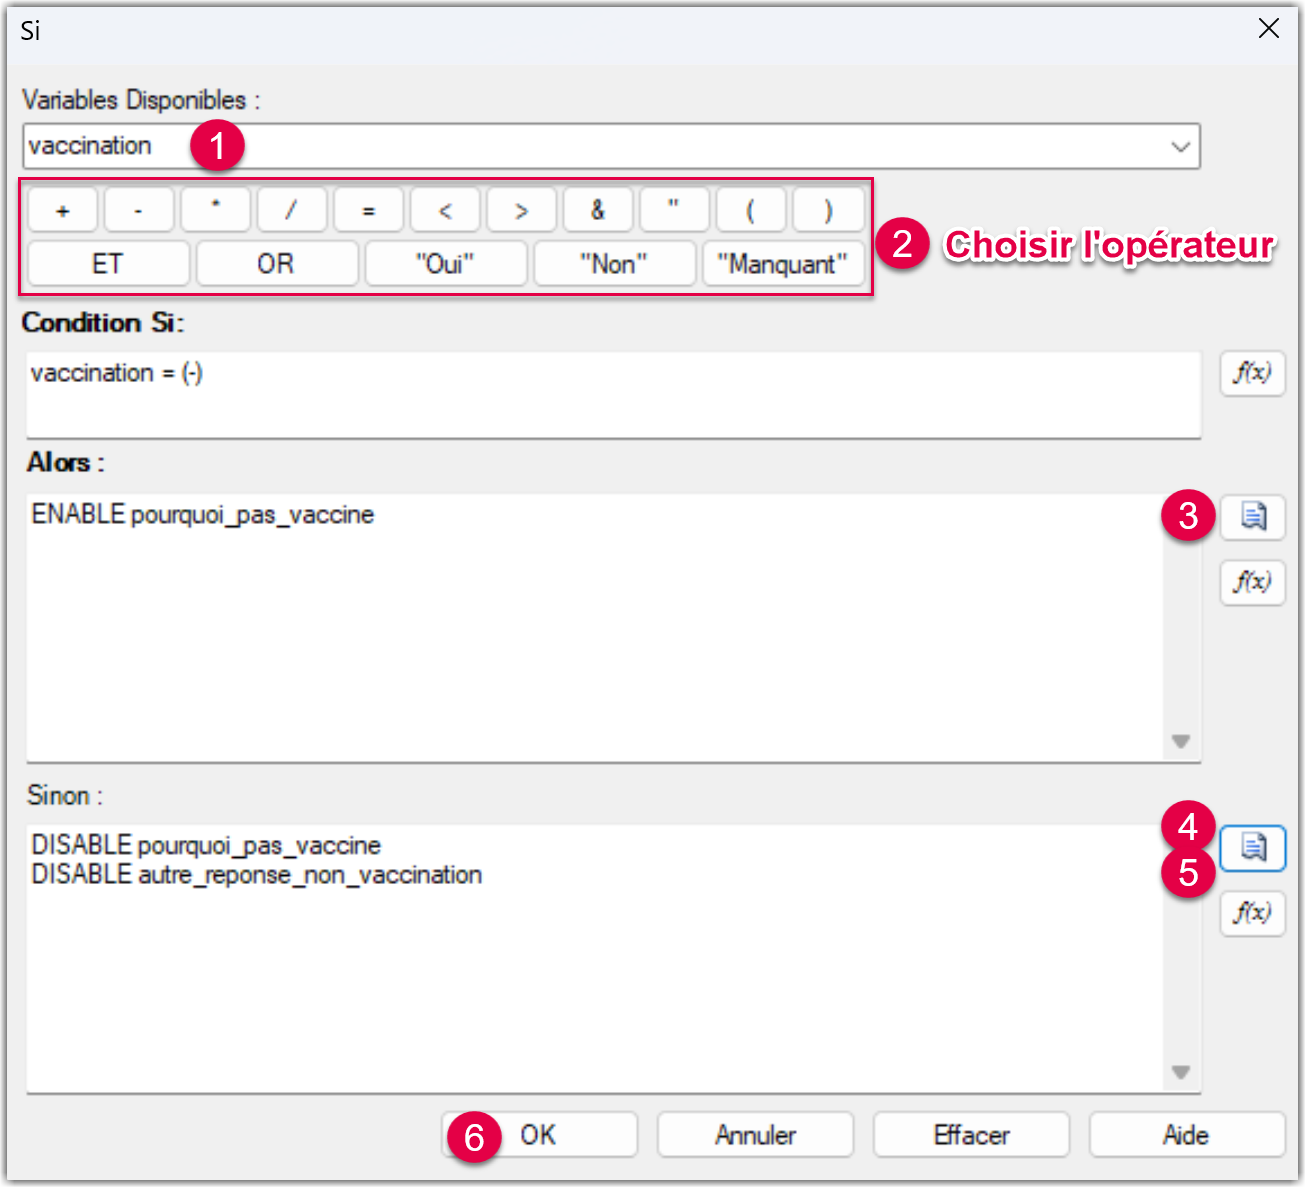
\includegraphics[width=\linewidth,height=0.4\textheight,keepaspectratio]{img/CodeValidation/codeIfEnableDisable}
	\caption{Création de code avec les commandes If, Enable et Disable}
	\label{fig:codeifenabledisable}
\end{figure}

Nous procédons de la même façon pour la variable \var{pourquoi\_pas\_vaccine} (\autoref{fig:codesipasvaccine}). Les codes obtenus s'affichent dans l'éditeur de programme (\autoref{lst:if}, page~\pageref{lst:if}, et \autoref{lst:ifelse}, page~\pageref{lst:ifelse}).

\begin{tcolorbox}[drop lifted shadow]
\begin{lstlisting}[language=EPIscript, style=mystyle, caption={Code de contrôle de la variable vaccination}, label=lst:if]
Field vaccination
	After
		//add code here
		IF vaccination = (-) THEN
			ENABLE pourquoi_pas_vaccine
		ELSE
			DISABLE pourquoi_pas_vaccine
			DISABLE autre_reponse_non_vaccination
		END-IF
	End-After
End-Field
\end{lstlisting}
\end{tcolorbox}

\begin{mybox}[colbacktitle=NOTE]{\faInfoCircle{} À RETENIR}
Dans le code de contrôle, la réponse \kw{Oui} d'un champ Oui/Non s'écrit \commande{(+)} et la réponse \kw{Non} s'écrit \commande{(-)}. Les boutons \kw{"Oui"} et \kw{"Non"} de la fenêtre \kw{Si} les insèrent automatiquement. La condition \commande{vaccination = (-)} signifie donc : \og si la personne n'est pas vaccinée \fg{}.
\end{mybox}

\begin{figure}[H]
	\centering
	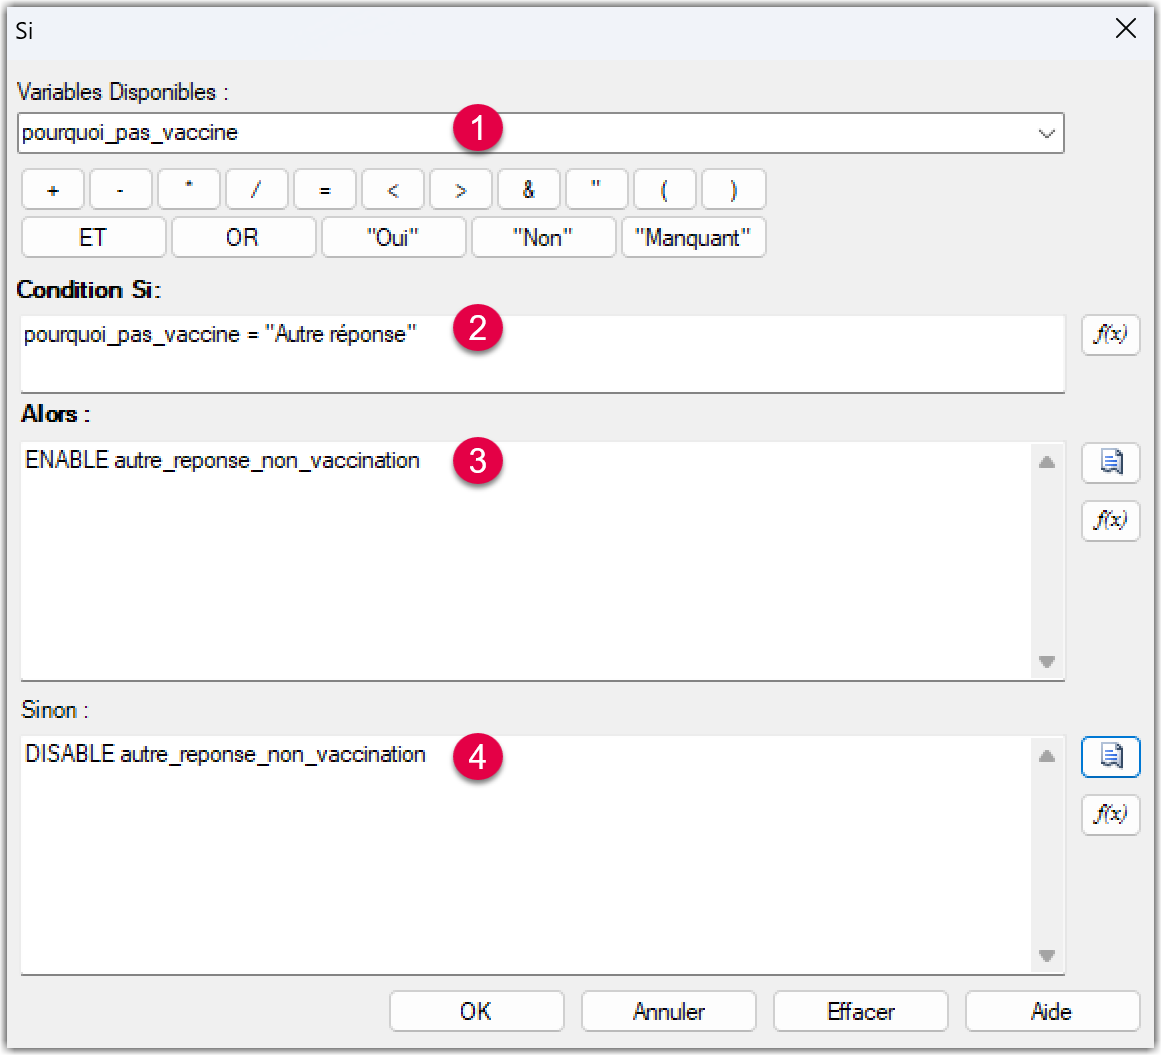
\includegraphics[width=\linewidth,height=0.4\textheight,keepaspectratio]{img/CodeValidation/codeSiPasVaccine}
	\caption{Activer le champ autre\_reponse\_non\_vaccination}
	\label{fig:codesipasvaccine}
\end{figure}

\begin{tcolorbox}[drop lifted shadow]
	\begin{lstlisting}[language=EPIscript, style=mystyle, caption={Code de contrôle de la variable pourquoi\_pas\_vaccine}, label=lst:ifelse]
Field pourquoi_pas_vaccine
	After
		//add code here
		IF pourquoi_pas_vaccine = "Autre réponse" THEN
			ENABLE autre_reponse_non_vaccination
		ELSE
			DISABLE autre_reponse_non_vaccination
		END-IF
	End-After
End-Field
	\end{lstlisting}
\end{tcolorbox}

\begin{mybox}[colbacktitle=CAUTION]{\faFire{} AVERTISSEMENT}
N'oubliez pas les guillemets droits \textcolor{IMPORTANT}{\texttt{"\,"}} pour délimiter une chaîne de caractères (du texte brut, par opposition à un nom de variable) lorsque vous faites une comparaison, comme dans \commande{IF pourquoi\_pas\_vaccine = "Autre réponse"}. Le texte doit être écrit exactement comme dans la liste des valeurs légales, accents et majuscules compris.
\end{mybox}

Comme vous pouvez le constater, le code de contrôle est un outil puissant. Il rend le questionnaire plus robuste et réduit les erreurs de saisie. Son apprentissage peut sembler rebutant au début, mais sa maîtrise vous ouvrira de nombreuses possibilités. Il n'est pas indispensable à la création d'un questionnaire, mais nous vous le recommandons vivement.
